\documentclass[11pt, oneside]{article}   	% use "amsart" instead of "article" for AMSLaTeX format
\usepackage{geometry}                		% See geometry.pdf to learn the layout options. There are lots.
\geometry{letterpaper}                   		% ... or a4paper or a5paper or ... 
%\geometry{landscape}                		% Activate for rotated page geometry
%\usepackage[parfill]{parskip}    		% Activate to begin paragraphs with an empty line rather than an indent
\usepackage{graphicx}				% Use pdf, png, jpg, or eps§ with pdflatex; use eps in DVI mode
								% TeX will automatically convert eps --> pdf in pdflatex		
\usepackage{amssymb}
\usepackage{amsmath}
\usepackage{float}
%SetFonts
\usepackage{tikz}
\usepackage{ragged2e}
\usepackage{adjustbox}
\usepackage{blindtext}
%\usepackage{romannum}
\usepackage[utf8]{inputenc}
\newcommand{\Var}{\operatorname{Var}}
% Default fixed font does not support bold face
\DeclareFixedFont{\ttb}{T1}{txtt}{bx}{n}{12} % for bold
\DeclareFixedFont{\ttm}{T1}{txtt}{m}{n}{12}  % for normal
\usepackage{enumitem}
% Custom colors
\usepackage{color}
\definecolor{deepblue}{rgb}{0,0,0.5}
\definecolor{deepred}{rgb}{0.6,0,0}
\definecolor{deepgreen}{rgb}{0,0.5,0}

\usepackage{listings}
\newtheorem{theorem}{Theorem}
\newtheorem{definition}{Definition}
\newtheorem{proof}{Proof}

% Python style for highlighting
\newcommand\pythonstyle{\lstset{
language=Python,
basicstyle=\ttm,
otherkeywords={self},             % Add keywords here
keywordstyle=\ttb\color{deepblue},
emph={MyClass,__init__},          % Custom highlighting
emphstyle=\ttb\color{deepred},    % Custom highlighting style
stringstyle=\color{deepgreen},
frame=tb,                         % Any extra options here
showstringspaces=false            % 
}}


% Python environment
\lstnewenvironment{python}[1][]
{
\pythonstyle
\lstset{#1}
}
{}

% Python for external files
\newcommand\pythonexternal[2][]{{
\pythonstyle
\lstinputlisting[#1]{#2}}}

% Python for inline
\newcommand\pythoninline[1]{{\pythonstyle\lstinline!#1!}}

\title{Machine learning and signal processing methods for anomaly detection in predictive maintenance (Project outline)}
\author{Yapi Donatien Achou}
%\date{}							% Activate to display a given date or no date

\begin{document}


\maketitle
\tableofcontents
\newpage
%\begin{figure}[H] %  figure placement: here, top, bottom, or page
%   \centering
%   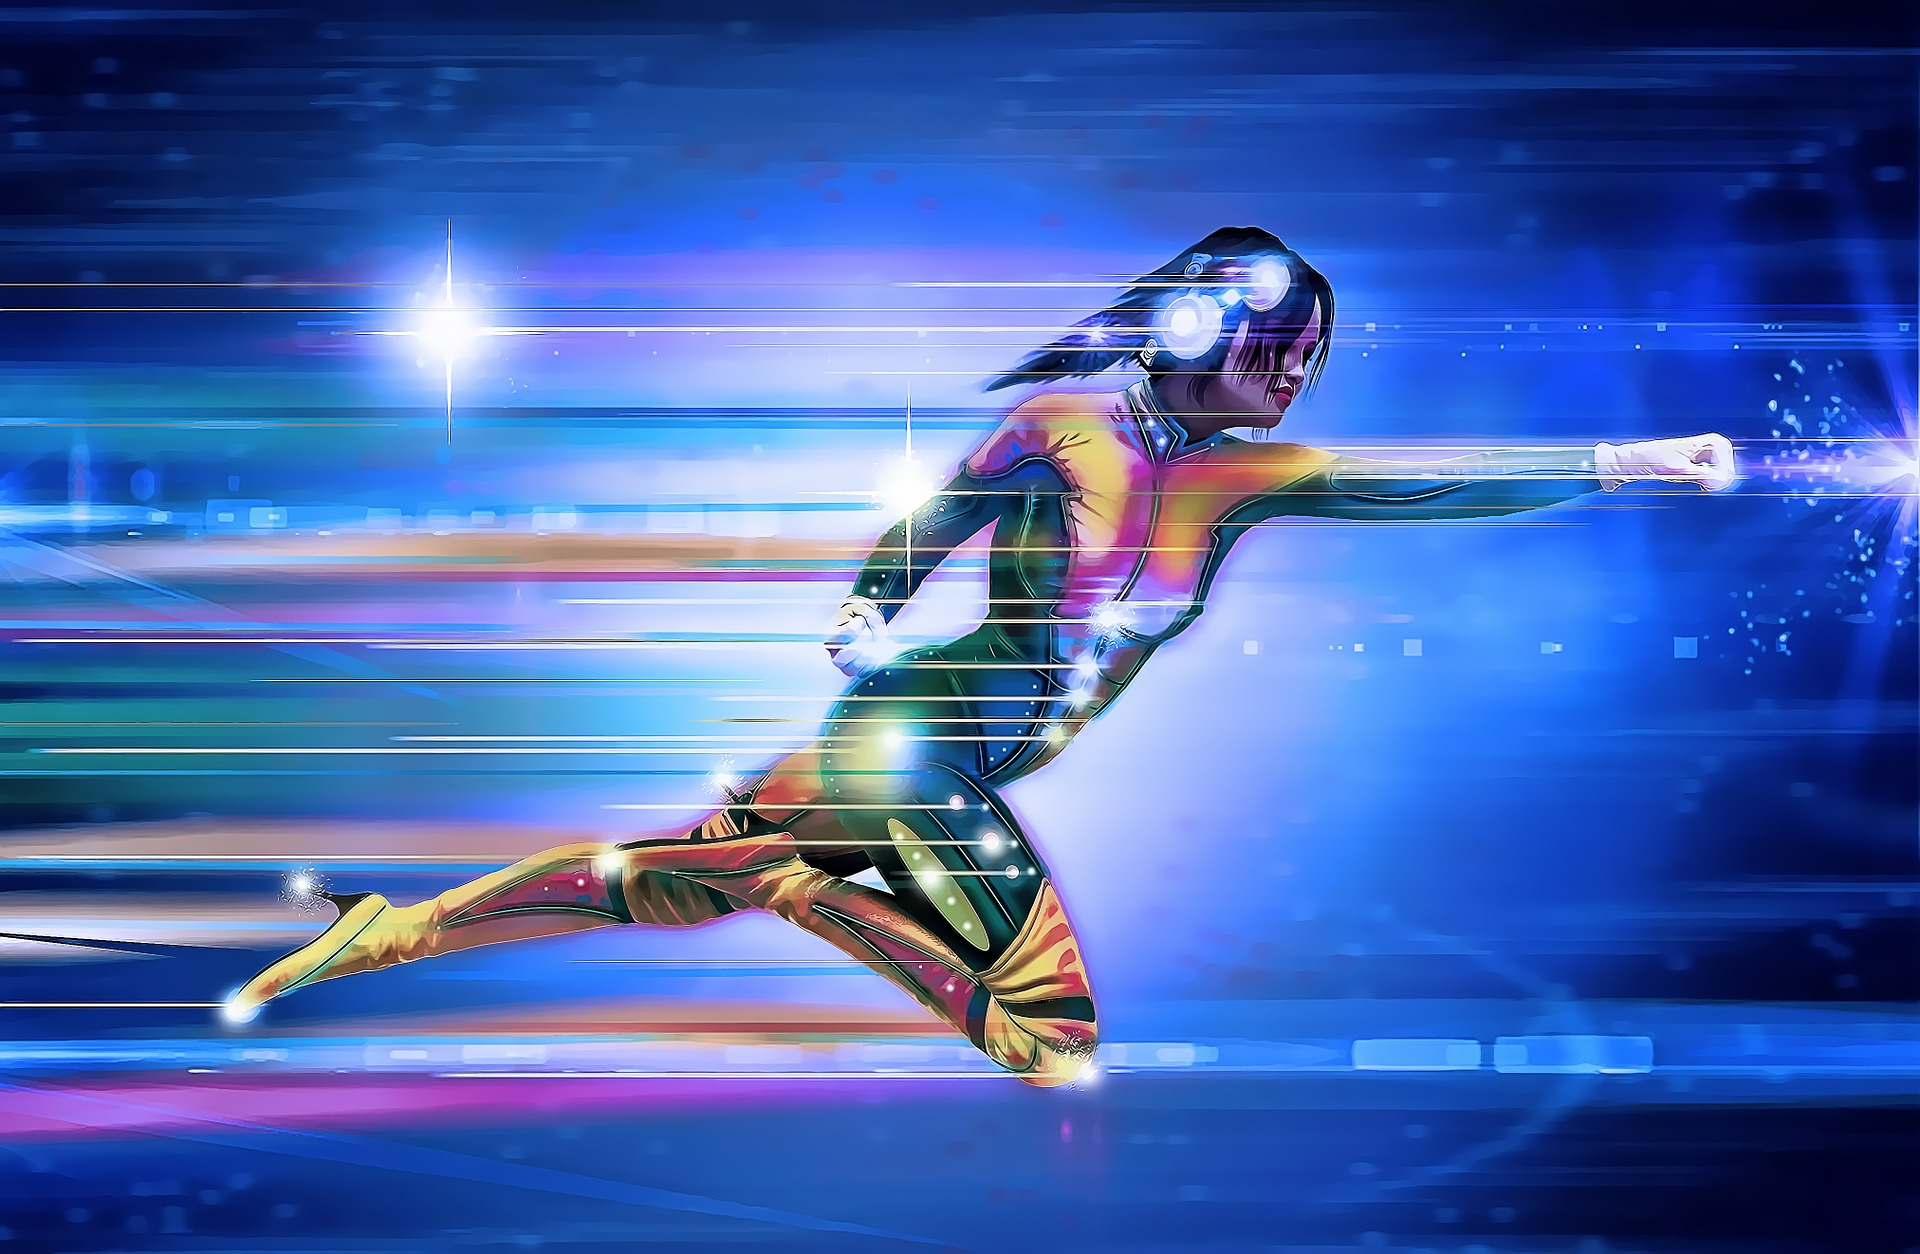
\includegraphics[width=5in]{front4} 
%   \caption{}
%   \label{fig:example}
%\end{figure}
\section{Introduction}
Since the industrial revolution, engines and machines have been the driving force for economical growth across industries such as automotive, airline, oil and gaze, to name a few. However, machines are prone to failure and must be monitor and maintain regularly to avoid catastrophic failure leading to significant financial and human lost. To mitigate equipment and machines proclivity toward failure and the associated cost, a process called predictive maintenance has been developed within the industrial community. Predictive maintenance  for machines and industrial equipments can be defined as a maintenance philosophy or more generally a framework with a set of methods used to predict and prevent machine failure in order to avoid unexpected downtime and reduce related human and financial cost. This maintenance philosophy, when correctly implemented, increases machine life time, and reduces maintenance cost [reference].
\justify
As a framework, predictive maintenance has 4 levels [reference]. In level 1, visual inspection of machines or equipments are performed in order to assess any damage.
In addition, equipment must fail before they are replaced, which can incur a high production cost. In level 2 and 3, machines characteristics such as vibration, temperature, electrical current, voltage etc are monitored continually or periodically depending on their criticality. This is called condition monitoring. In condition monitoring, the goal is to detect any change in machine normal behaviour, in order to detect failure as early as possible and schedule maintenance accordantly. Maintenance actions are performed periodically regardless of machine health condition. In level 4, big data and machine learning are the main driving forces in detecting failure and planning maintenance. At this level, maintenance action are not performed periodically but are planned according to machine health condition derived from the application of anomaly detection techniques. This reduce unnecessary maintenance action and significantly cut down maintenance cost as well as increasing machine life time.
\justify
According to PriceWaterhouseCoopers (PWC), one of the four largest auditing and consulting company in the world,  a survey from 280 companies in Belgium, Germany and the Nederland, revealed that only 
$11 \%$ of companies have reached level 4 \cite{pwc}. The application of level 4 requires collecting, saving and analysing large amount of data, from which maintenance decision can be made. Anomaly detection methods and more generally supervised and unsupervised learning methods are used in the analysis phase.
%These methods, detect early sign of anomalies such as machines defect and predict their remaining useful life, which is the time left before catastrophic break down. 
\justify
In supervised learning, based on available failure data from defect machine, a learning algorithm is trained to recognise the failure pattern in the data. This is sometime achieved by fitting the algorithm parameters to the data, which result in a model called a classifier or a regressor. A classifier is a model derived from a classification algorithm while a regressor is a model derived from a regression algorithm.
\justify
 In machine learning, the failure data is called a labeled data because we can assign a categorical label such as fail or a numerical label such as 1 to specify the condition of the machine through the data measuring its characteristics. In the absence of labeled data, unsupervised learning methods can be apply to detect pattern in the data without prior knowledge to classify data regions as anomalous or not. One such technique is clustering algorithm where the input data is separated into subregions.
\justify
The procedure of classifying a data region as anomalous or not is called anomaly detection. An anomaly is defined as a pattern in the data, that does not conform to expected normal behaviour \cite{chandola}. A general anomaly detection strategy will first detect normal behaviour, secondly set a boundary around the normal behaviour and finally declare any data out of the boundary as anomaly.
\justify
Several factor make this general approach of anomaly detection challenging: The notion of anomaly is different for different application domain and not all application domain have enough labeled data to train a supervise learning algorithm \cite{chandola}. An extensive survey from \cite{chandola} revealed that the majority of research have been focussing on simple anomalies while most application domain are faced with complex anomalies. There are mainly three types of anomalies: Point anomalies which are simple anomalies, contextual  and collective anomalies which are complex anomalies \cite{chandola}. When one data point in a time series is anomalous with respect to the other data points, we have a point anomaly. In a contextual anomaly, a data instance is anomalous relative to a context. For example the vibration of a machine might be very high if the load increase suddenly, and decrease when the load goes back to normal. But if the vibration increases monotonously regardless of the load, then we have a contextual anomaly. If a collection of related data instance is anomalous with respect to the entire data set, it is termed a collective anomaly \cite{chandola}.


\begin{flushleft}
In rotating machines, more than 40 $\%$ of anomalies can be attributed to bearing defect [references]. Figure \ref{fig:pie} shows the failure statistics for rotating machines. 
\end{flushleft}
\begin{figure}[H] %  figure placement: here, top, bottom, or page
   \centering
   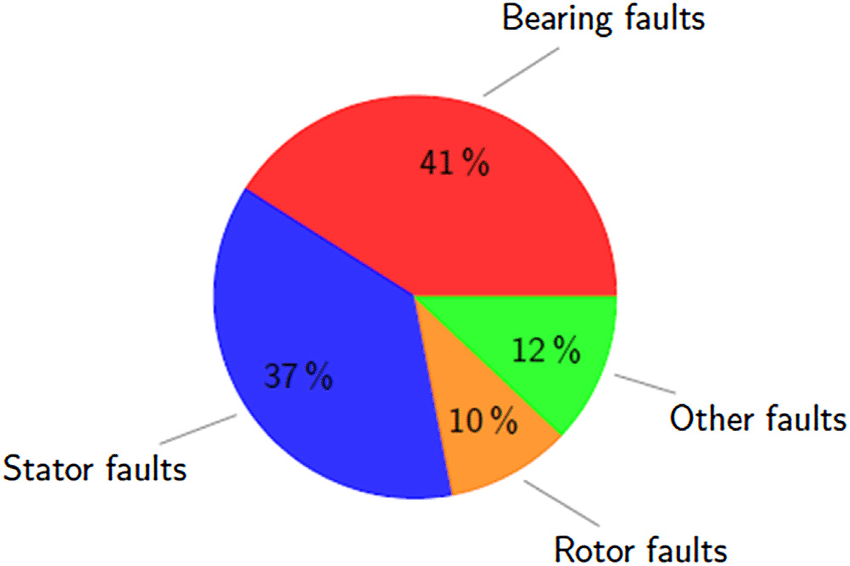
\includegraphics[width=5in]{pie.png} 
   \caption{Defect statistics for rotating machines, taken from [reference]}
   \label{fig:pie}
\end{figure}
In this project we present a mixed methodology to detect and predict bearing defects. The methodology consists of using signal processing for feature generation and data labelling,  and machine learning for defects classification and failure prediction. For a given input dataset, the dataset is decomposed into it subcomponents or basis components. The basis components also called features or attributes are further used as input of a supervised learning algorithm for defect classification and failure prediction.
\begin{flushleft}
The signal processing methods used are Fourier transform, wavelet transform and Hilbert Huang transform. We focus on ensemble learning and feed forward neural network for classification. Furthermore we show that the back-propagation process in the feed forward neural network can be modelled by an ordinary differential equation, whose solution represents the path of the hidden and output layer weights.
\end{flushleft}
\justify
This thesis is structured into six parts. To put the current work in prospective, chapter two outlines preview works, where machine learning and/or signal processing have been applied to anomaly detection for machines fault detection. Since the latter is the main goal, chapter three presents a general anomaly detection methodology, followed by a proposed methodology for predictive maintenance. The main methods used for anomaly detection, that is signal processing and machine learning are presented in chapter four and five respectively. The capstone of this work, to say the least, is revealed in chapter six in a form of three case studies, where we apply our proposed methodology to solve up to date anomaly detection problems encounter in a wide range of industries.
As in any work, we conclude this thesis by summarising what have been done. The summary includes the strengths and weaknesses of our methodology, as well as what could be done to improve upon it.


%%%%%%%%%%%%%%%%%%%%%%%%%%%%%%%%%%%%%%%%%%%%%%%%%%%%%%%%%%%%%%%%%%%%%%%%%%%%%%%%%%%%
%%%%%%%%%%%%%%%%%%%%%%%%%%%%%%%%%%%%%%%%%%%%%%%%%%%%%%%%%%%%%%%%%%%%%%%%%%%%%%%%%%%%
%%%%%%%%%%%%%%%%%%%%%%%%%%%%%%%%%%%%%%%%%%%%%%%%%%%%%%%%%%%%%%%%%%%%%%%%%%%%%%%%%%%%

\section{Literature review  \textcolor{red}{(TO DO!!)})}

%%%%%%%%%%%%%%%%%%%%%%%%%%%%%%%%%%%%%%%%%%%%%%%%%%%%%%%%%%%%%%%%%%%%%%%%%%%%%%%%%%%%
%%%%%%%%%%%%%%%%%%%%%%%%%%%%%%%%%%%%%%%%%%%%%%%%%%%%%%%%%%%%%%%%%%%%%%%%%%%%%%%%%%%%

\section{Anomaly detection methodology and methods \textcolor{red}{(TO DO!!)}}
\subsection{General anomaly detection methodology   \textcolor{red}{(TO DO!!)}}
\subsection{A proposed methodology for predictive maintenance   \textcolor{red}{(TO DO!!)}}

%%%%%%%%%%%%%%%%%%%%%%%%%%%%%%%%%%%%%%%%%%%%%%%%%%%%%%%%%%%%%%%%%%%%%%%%%%%%%%%%%%%%
%%%%%%%%%%%%%%%%%%%%%%%%%%%%%%%%%%%%%%%%%%%%%%%%%%%%%%%%%%%%%%%%%%%%%%%%%%%%%%%%%%%%




%%%%%%%%%%%%%%%%%%%%%%%%%%%%%%%%%%%%%%%%%%%%%%%%%%%%%%%%%%%%%%%%%%%%%%%%%%%%%%%%%%%%
%%%%%%%%%%%%%%%%%%%%%%%%%%%%%%%%%%%%%%%%%%%%%%%%%%%%%%%%%%%%%%%%%%%%%%%%%%%%%%%%%%%%


\section{Signal processing methods}
\subsection{Overview}
 In this section, we present three signal processing methods to generate new features also called attributes, for anomaly detection. In the context of this work, a feature or attribute is a numerical sequence that represents the state of a system. For example, voltage and vibration measurement taken from a motor over time are time series that we call features. These two features contain information about the state of the motor, the latter being the system in this case. 
 By state we mean the current health of the motor. The health of the motor is represented by a health index which is a numerical value that quantifies the overall condition of the motor.
 \justify
 Generating new features from existing one, is a common procedure for anomaly detection. For example, by using Fourier transform, we can generate the frequency spectrum of a vibration time series. The frequency spectrum is the set of all frequencies from each vibration component of the original vibration time series. The importance of the frequency spectrum, lies in the fact that if a motor or machine is anomalous, the anomaly will generate an extra component in the vibration time signal, and the corresponding anomalous frequency will be visible in the frequency spectrum. Due to Fourier transform limitations, other signal processing techniques such as
  wavelet and Hilbert Huang transform are alternatives for generating new features to deal with more complex time series for anomaly detection.
 \justify
 In the rest of this section, we give an expos$\acute{e}$  of three signal processing methods, namely: Fourier transform, wavelet transform and Hilbert Huang transform. For each transform, we cover the theoretical back bone in terms of mathematical constructs such as basis, vector space, orthogonality, existence, uniqueness, to name a few. Furthermore, these mathematical constructs will set the limitations as well as the strengths of each transform. Following the theoretical set up is a concrete application, where we generate new features and show how they can be used for anomaly detection.
 
%%%%%%%%%%%%%%%%%%%%%%%%%%%%%%%%%%%%%%%%%%%%%%%%%%%%%%%%%%%%%%%%%
%%%%%%%%%%%%%%%%%%%%%%%%%%%%%%%%%%%%%%%%%%%%%%%%%%%%%%%%%%%%%%%%%


\subsection{Fourier Analysis}
\subsubsection{Theory}
Fourier analysis is concerned with the general problem of functions approximation. The basic ingredients required to approximate a function are: a vector space, a basis, which is a subspace of the vector space and a mathematical operation or more generally a function such as an inner product that maps two vectors to a real number. If a vector space has an inner product, we say that the vector space is an inner product space. 
\justify
The function approximation process goes like this: We select an arbitrary function $f$. We pick an appropriate vector space which we call $V$, such that $f\in V$. We define a subspace $V_{0}$ of the vector space $V$ and construct an inner product on $V_{0}$, if it does not exist. Furthermore, we fine an appropriate basis of $V_{0}$.  A basis of $V_{0}$ is a set of linearly independent vectors say $\varphi_{j}$ in $V_{0}$, conveniently denoted by $\{ \varphi_{j}\}_{j=0}^{n}$ that span $V_{0}$. This means that any vector in $V_{0}$ can be written as a linear combination of the basis vectors. Once we have all this in place, then the best approximation of the function $f$ is its orthogonal projection in the inner product space $V_{0}$. Figure \ref{figure:il} shows an illustration of function approximation.
\justify
\begin{figure}[H]
\begin{center}
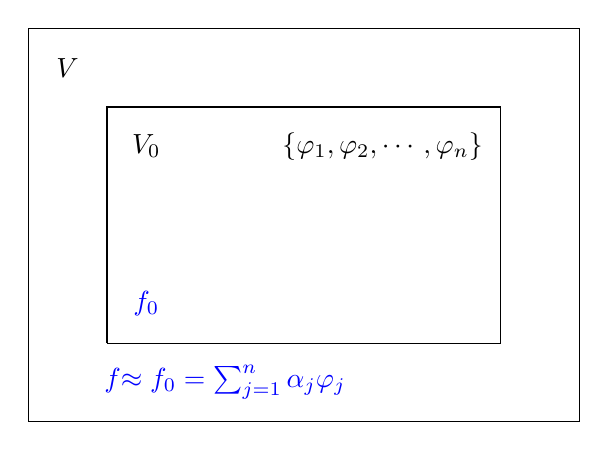
\begin{tikzpicture}
%\draw (0,0) -- (0,5) -- (0,0) -- (5,0) -- (5,5) -- (0,5);
%\draw (1,1) -- (1,4) -- (1,1) -- (4,1) -- (4,4) -- (1,4);
%\draw (0,0) rectangle (7,5);
%\draw (1,1) rectangle (6,4);
% reactagle 1
\path (0,0) coordinate (origin1);
\path(0.5,4.5) node (V){$V$};
\path(2.5,0.5) node (f){$\textcolor{blue}{f}\textcolor{blue} {\approx f_{0} = \sum_{j=1}^{n} \alpha_{j} \varphi_{j}}$};
\path (0,5) coordinate (topleft1);
\path (7,5) coordinate (topright1);
\path (7,0) coordinate (bottom1);
% draw
\draw (origin1) -- (bottom1) -- (topright1) -- (topleft1) -- (origin1);

% reactagle 2
\path (1,1) coordinate (origin2);
\path(1.5,3.5) node (V0){$V_{0}$};
\path(1.5,1.5) node (f0){$\textcolor{blue}{f_{0}}$};

\path (1,4) coordinate (topleft2);
\path (6,4) coordinate (topright2);
\path(4.5,3.5) node (b0){$ \{\varphi_{1}, \varphi_{2}, \cdots, \varphi_{n}\} $};
\path (6,1) coordinate (bottom2);
% draw
\draw (origin2) -- (bottom2) -- (topright2) -- (topleft2) -- (origin2);
\end{tikzpicture}
\end{center}
\caption{Illustration of a generic function approximation process of a function $f$ into a subspace $V_{0}$ of a vector space $V$. $\varphi_{j}$ are the basis function and $\alpha_{j}$ are real numbers for $j=1,\cdots,n$.}
\label{figure:il}
\end{figure}
\justify
Let have a closer look at each ingredient and define further properties that make Fourier analysis an appropriate tool for function approximation. We shall shortly define the concepts of vector space, basis, inner product, orthogonality and additional properties that are derived from them.
\begin{definition}
A vector space $V$ over a field $F$ is a set  with two operations $(\cdot, +)$ satisfying 
\begin{enumerate}
\item Associativity:  (u+v)+w = u+(v+w), for any u,v, w $\in V$
\item Commutativity: u+v = v+u, for all u,v $\in V$
\item Inverse: for any u $\in V$ there exists an element -u $\in V$ such that u + (-u) = 0
\item Identity element: $1\cdot u = u$ where 1 is the multiplicative identity in he field F.
\item Distributivity: $a\cdot(u+v) = a\cdot u + a\cdot v$, for any a $\in F$, and u, v $\in V$
\item Compatibility $a\cdot(b\cdot u) = (a\cdot b)\cdot u$, for any a,b $\in V$ and u $\in V$
\item Scalar distributivity $(a+b)\cdot u = a\cdot u + b\cdot u$, for any a,b $\in F$, and u $\in V$
\end{enumerate}
The elements of the vector space V are called vectors and the element of the field F are call scalars.
\end{definition}
An example of an inner product space is the $L^{2}$ space which encompasses square integrable functions. By definition, the set of all squared integrable functions on an interval say $[0,T]$ is denoted by 
$L^{2}[0,T]$. Any real function $f$ in $L^{2}[0,T]$ satisfies
\begin{equation} \label{eq:L2}
\int_{0}^{T}f(t)^{2}\mathrm{d}t < \infty.
\end{equation}
For two functions $f$ and $g$ in $L^{2}[0,T]$, we define their inner product as 
\begin{equation}
\langle\ f,g \rangle = \frac{1}{T}\int_{0}^{T}f(t)g(t)\mathrm{d}t.
\end{equation}
Equation (\ref{eq:L2}) says that the total energy of $f$ is finite. This suggest that the $L^{2}$ space is important for real world applications such as signal processing. In fact, we will see  later in more detail that any function in $L^{2}$ has a Fourier expansion given in terms of linear combination of sinusoidal basis functions. 
\justify
A legitimate question that comes in mind is, how are vectors organised in a vector space. One way to organise vectors in a vector space is to define them in terms of special set of vectors called basis, having well defined properties. Each vector will then be uniquely expressed in terms of the basis vectors. 
\justify
\begin{definition}
A basis is a set of vectors $\varphi_{i}, i = 1, \cdots, n$, covenantally written as 
\begin{equation}
\{ \varphi_{1}, \cdots, \varphi_{n} \} \nonumber,
\end{equation}
that spans the whole vector space and is linearly independent. Spanning the whole space means that for any vector u $\in V$ there exist unique scalars $a_{i}$ where $i=1,\cdots,n$, such that 
\begin{equation}
u = a_{1}\varphi_{1} + \cdots + a_{n}\varphi_{n} \nonumber,
\end{equation}
and linearly independent means that if
\begin{equation}
a_{1}\varphi_{1} + \cdots + a_{n}\varphi_{n} = 0 \nonumber,
\end{equation}
then 
\begin{equation}
a_{1} = \cdots = a_{n} = 0 \nonumber
\end{equation}
\end{definition}
\justify
With a given basis we can uniquely approximate a vector by decomposing its in terms of the basis vectors. However, a vector space can have several basis, giving rise to several approximations of the same vector. In mathematics and in science in general, one is often concerned with the optimum solution or the unique solution. In terms of an application, uniqueness allows one to pick the relevant physical solution.
It turns out that, regardless of the basis, the orthogonal projection of a vector is its optimum approximation. Orthogonal projection is achieved by a special operation called inner product. Let formally define an inner product and show how its define orthogonality.

\begin{definition}
An inner product on a real vector space $V$ is a function 
\begin{equation}
\langle\,,\rangle : V\times V \rightarrow \mathbb{R} \nonumber
\end{equation}
that satisfies the following properties $\forall u,v \in V$
\begin{enumerate}
\item Positivity: $\langle\ u,v \rangle > 0$, \quad 
\item Symmetry: $\langle\ u,v \rangle > 0  = \langle\ u,v \rangle$
%\item Homogeneity:
%\item Linearity:
\end{enumerate}
A vector space with an inner product is called an inner product space.
\end{definition}
\vdots
\vdots
\textcolor{red}{(NEED TO EXPAND MORE HERE AFTER THE DEFINITION)})
\begin{definition}
Suppose $V$ is an inner product space.
\begin{itemize}
\item The vectors $u$ and $v$ are orthogonal if $\langle\ u,v \rangle = 0$
\item A finite set of vectors $\{ v_{j} \}_{j=1}^{n}$ are orthonormal if each vector have unit length with respect to a norm $||, ||$, that is 
\begin{equation}
||v_{j}|| = 1 \nonumber
\end{equation}
and $v_{i}$ and $v_{j}$ are orthogonal for $i\neq j$ 
\end{itemize}
\end{definition}
\vdots
\vdots
\textcolor{red}{(NEED TO EXPAND MORE HERE AFTER THE DEFINITION)}

\begin{definition}
Suppose $V_{0}$ is a finite-dimensional subspace of an inner product space $V$. For any vector $v \in V$, the orthogonal projection of $v$
into $V_{0}$ is the unique vector $v_{0} \in V_{0}$ that is closest to $v$, that is,
\begin{equation}
 ||v-v_{0}|| =  \min_{\forall w \in V_{0}} || v-w ||,
\end{equation}
\end{definition}
\vdots
\vdots
\textcolor{red}{(NEED TO EXPAND MORE HERE AFTER THE DEFINITION)}
\begin{theorem}\label{orthogonalityTheorem}
Suppose $V_{0}$ is a  n-dimensional subspace of an inner product space $V$ and let $\{  \varphi_{j} \}_{j=1}^{n}$ be an orthonormal basis for $V_{0}$, then the orthogonal projection
of a vector $v\in V$ onto $V_{0}$ is given by 
\begin{equation}
v = \sum_{j=1}^{n}\alpha_{j}\varphi_{j}, \quad \text{where}, \quad \alpha_{j} = \langle\ v,\varphi_{j} \rangle \in \mathbb{R}
\end{equation}
\end{theorem}

\begin{proof}
(Need a proof here) 
\end{proof}

\justify
From Theorem \ref{orthogonalityTheorem}, We saw that a vector can be decomposed in terms of basis functions by orthogonal projection. The orthogonal projection ensures that the decomposition is optimum with respect to a chosen basis. In Fourier analysis, the basis functions are trigonometric functions of period $2\pi$.
\begin{theorem}
The set of functions 
\begin{equation}
\left \{ \cdots, \frac{\cos(2x)}{\sqrt{\pi}},\frac{\cos(x)}{\sqrt{\pi}},\frac{1}{\sqrt{\pi}}, \frac{\sin(x)}{\sqrt{\pi}},\frac{\sin(2x)}{\sqrt{\pi}},\cdots  \right \}
\end{equation}
is an orthonormal set in $L^{2}([-\pi,\pi])$ space
\end{theorem}
\begin{proof}
(Need a proof here) 
\end{proof}
\textcolor{red}{(NEED TO EXPAND MORE HERE AFTER THE THEOREM)}
\begin{definition}
The Fourier series of a periodic function $g$ is given by the expansion 
\begin{equation}
g(x) = a_{0} + \sum_{k=1}^{n}a_{k}\cos(kx)+b_{k}\sin(kx)
\end{equation}
where $a_{k}, k=0,\cdots, n$ are called the Fourier coefficients of the function $g$
\end{definition}
\vdots
\vdots
\textcolor{red}{(NEED TO EXPAND MORE HERE AFTER THE DEFINITION)}
\begin{theorem}
if 
\begin{equation}
g(x) = a_{0} + \sum_{k=1}^{n}a_{k}\cos(kx)+b_{k}\sin(kx)
\end{equation}
then 
\begin{equation}
a_{0} = \frac{1}{2\pi}\int_{-\pi}^{\pi}g(x)\mathrm{d}x
\end{equation}
\begin{equation}
a_{k} = \frac{1}{2\pi}\int_{-\pi}^{\pi}g(x)\cos(kx)\mathrm{d}x
\end{equation}
\begin{equation}
b_{k} = \frac{1}{2\pi}\int_{-\pi}^{\pi}g(x)\sin(kx)\mathrm{d}x
\end{equation}
\end{theorem}

\begin{proof}
\vdots
\vdots
(need a proof here) We use the orthogonality property to derive the Fourier coefficients.
\end{proof}

\vdots
\vdots
\textcolor{orange}{TO BE CONTINUED}











\subsubsection{Application}
In this approach we use Fourier transform to detect defect frequency such outer race defect frequency and inner race defect frequency in the envelop spectrum. In this case the envelop spectrum is the new feature generated from the original vibration data. The bearing type used are Rexnor ZA-2115. For this type of bearing, the constant defect frequency (cdf) for ball pass frequency outer race defect is 0.1182 and the constant defect frequency for ball pass frequency inner race defect is 0.1484 [reference]. According to Rexnord product engineering group [reference], to find the defect frequency in Hz we multiply the constant defect frequency (cdf) by the rotational speed of the bearing ( here 2000 RPM), to find the defect frequency in Hz. Note that the defect frequency is computed from the geometry of the bearing, which means that for a specific bearing, this is a constant value. 

\begin{flushleft}
Figure \ref{fig:bearing} shows the geometry of a bearing, from which bearing defect frequency can be computed. Figure \ref{fig:decomp}  illustrates how Fourier transform can decompose vibration data into its frequency components. Each frequency component which are trigonometric functions are characterised by constant frequency and amplitude. In a defect bearing, the defect frequency will be coupled with a relatively high amplitude. 
\end{flushleft}
\begin{figure}[H] %  figure placement: here, top, bottom, or page
   \centering
   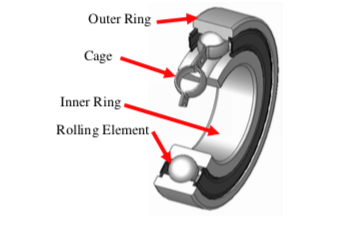
\includegraphics[width=4in]{bearing.png} 
   \caption{Geometry of a bearing}
   \label{fig:bearing}
\end{figure}
\begin{flushleft}
\begin{figure}[H] %  figure placement: here, top, bottom, or page
   \centering
   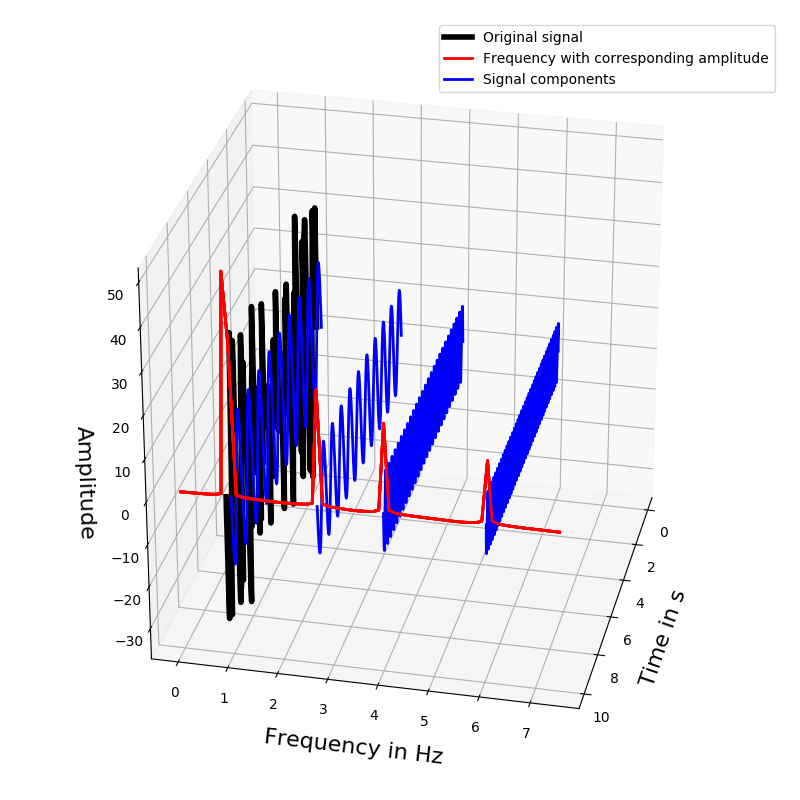
\includegraphics[width=4in]{decomposition} 
   \caption{Illustration of using Fourier transform to decompose a time signal to its frequency components}
   \label{fig:decomp}
\end{figure}

Next, we compute the envelop spectrum for each vibration signal by using the FFT method (Fast Fourier Transform). The envelop spectrum is used to detect early sign of failure. Recall that a vibration signal can be decomposed into its sub components, where each  sub component 
is characterised by its frequency and its amplitude. Early sign of failure can be seen in the high frequency low amplitude sub component. As the failure becomes more pronounced, it becomes visible in the low frequency high amplitude sub component. Figure \ref{fig:signal0} shows the raw vibration signal, the corresponding envelop spectrum and the ball pass frequency outer race defect.
\end{flushleft}

\begin{figure}[H] %  figure placement: here, top, bottom, or page
   \centering
   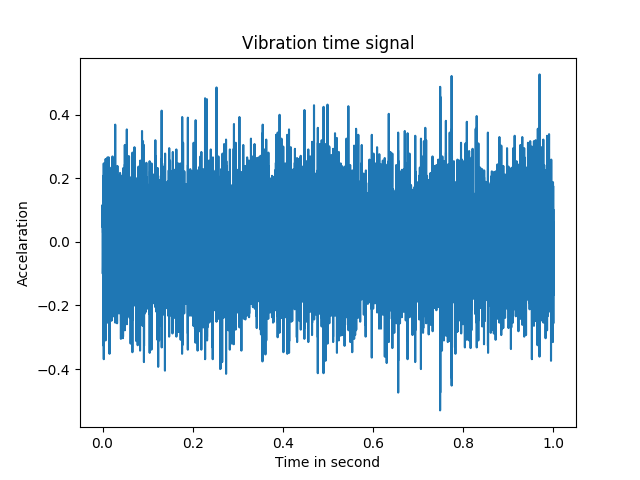
\includegraphics[width=4in]{time-signal.png} 
   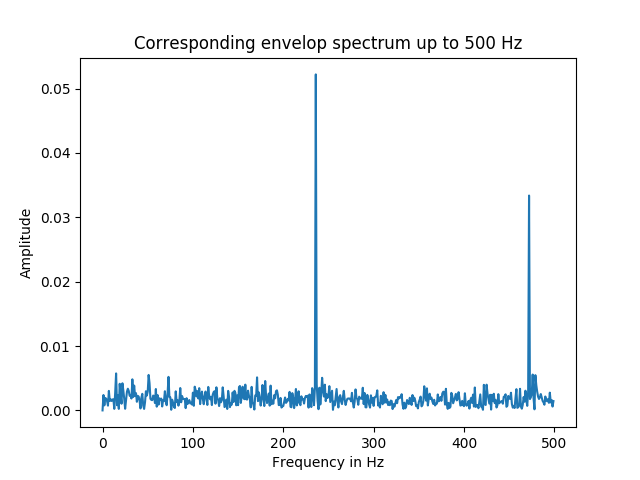
\includegraphics[width=4in]{spectrum.png} 
      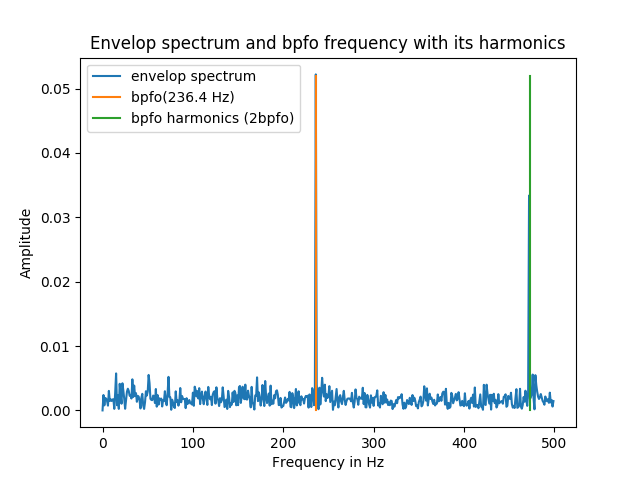
\includegraphics[width=4in]{fault.png} 
   \caption{Vibration time signal}
   \label{fig:signal0}
\end{figure}
\begin{flushleft}
By computing the envelop spectrum for each time signal and extracting the amplitude of a defect frequency we can visualise the severity of a defect. Figure \ref{fig:signal111} and \ref{fig:signal221} show the amplitude of outer race defect and inner race defect for four bearings and three bearings respectively. In Figure \ref{fig:signal111} we can observe that bearing number one is affected severely by ball pass frequency outer race defect. Figure \ref{fig:signal222} shows that bearing number three has ball pass frequency inner race defect. 
\end{flushleft}
\begin{figure}[H] %  figure placement: here, top, bottom, or page
   \centering
   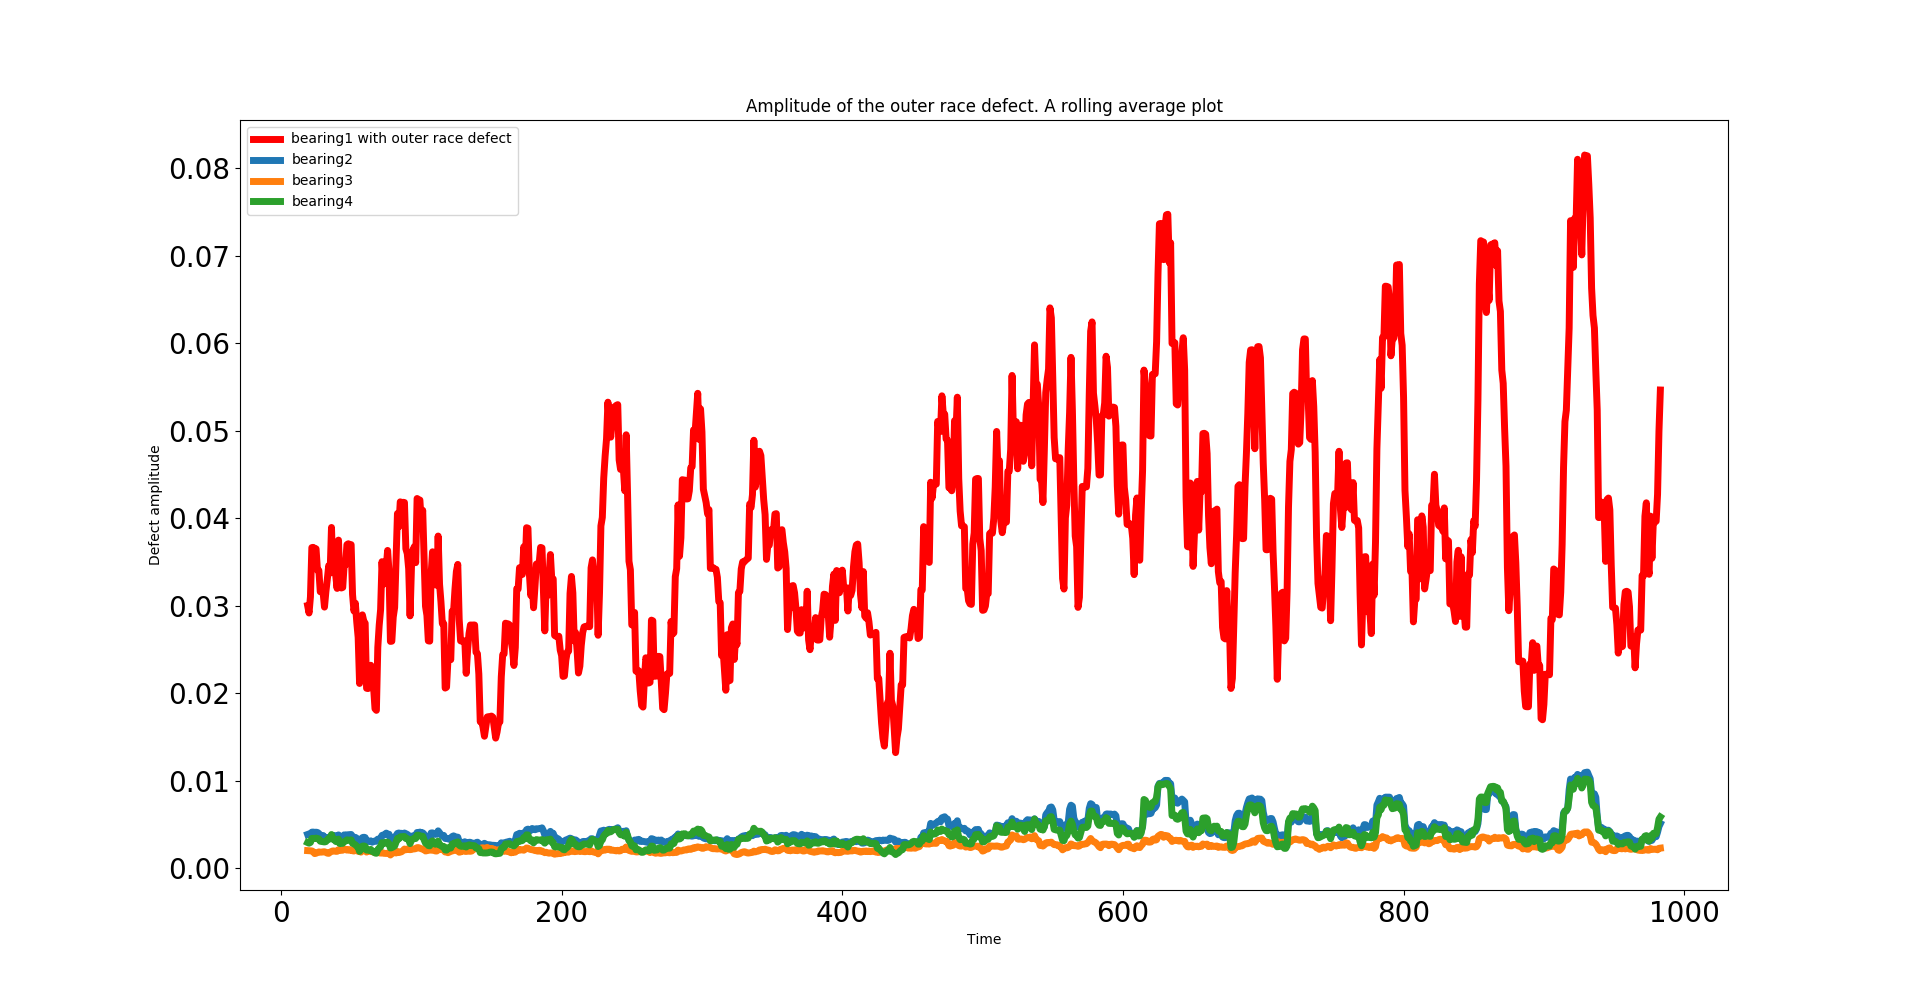
\includegraphics[width=7in]{signal_processing_method_bpfo} 
   \caption{Ball pass frequency outer race detection}
   \label{fig:signal111}
\end{figure}

\begin{figure}[H] %  figure placement: here, top, bottom, or page
   \centering
   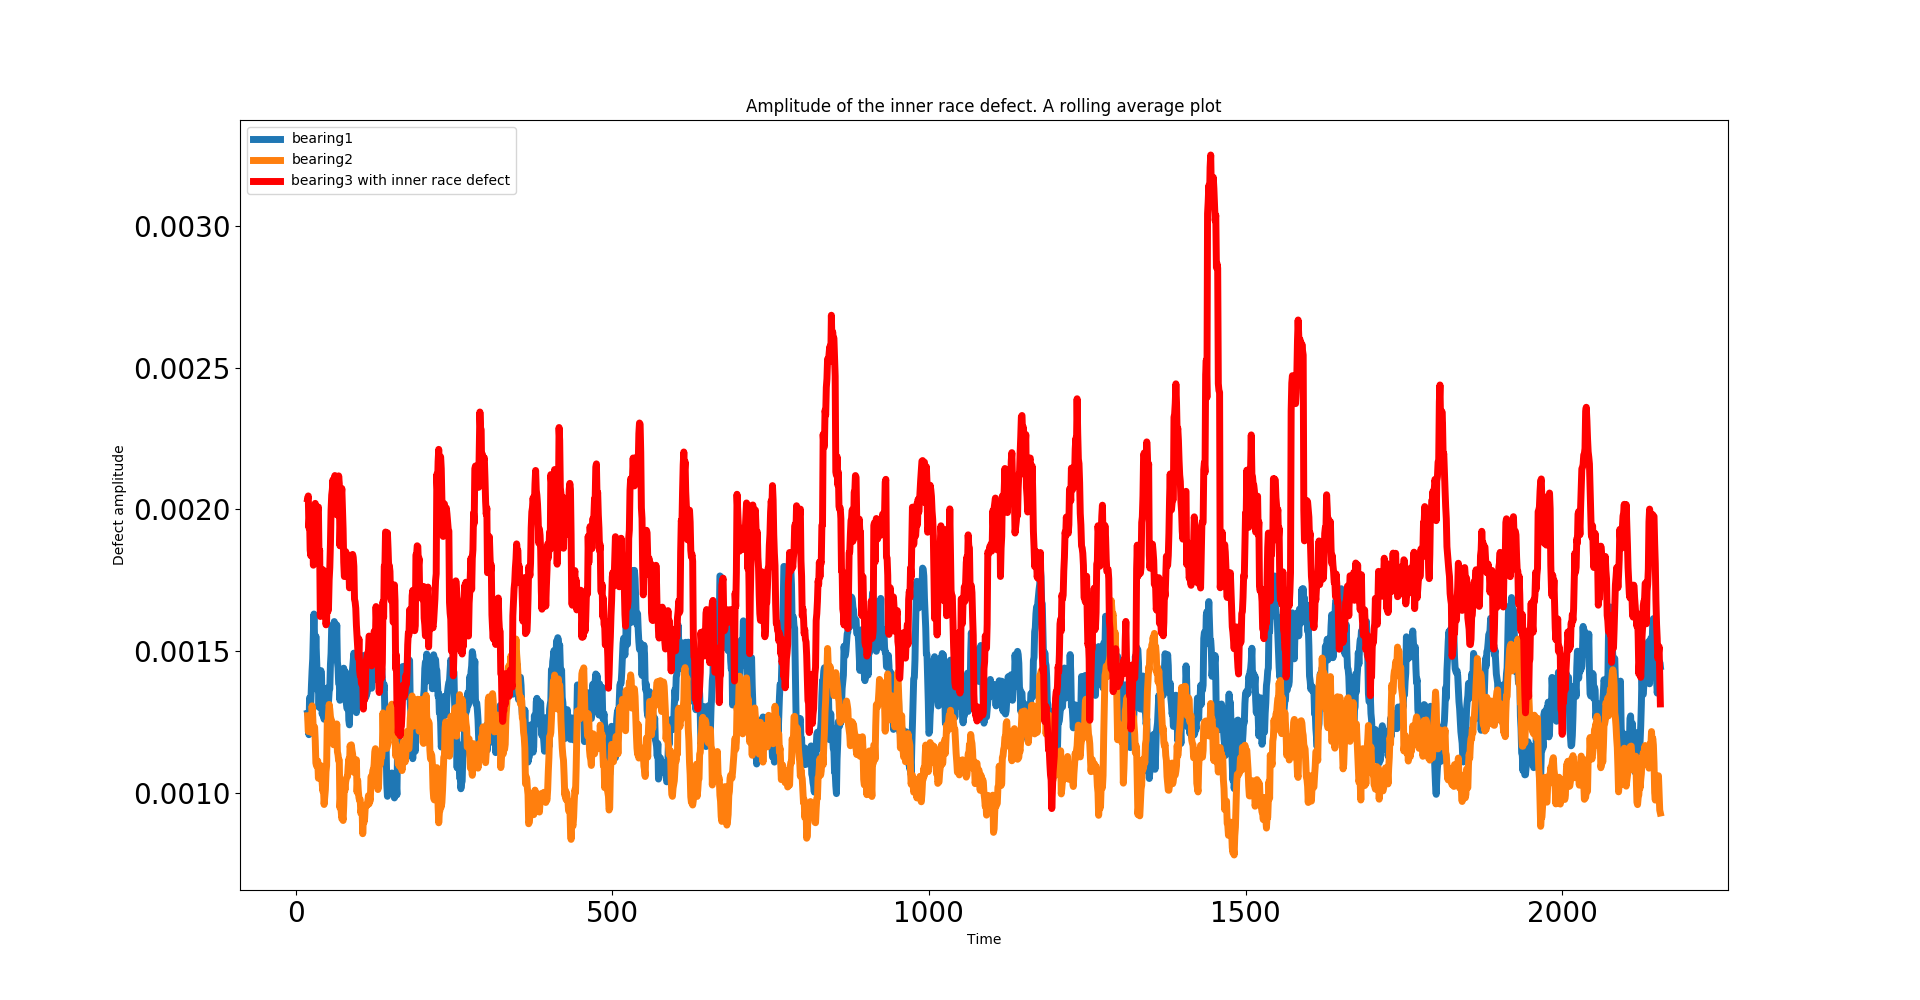
\includegraphics[width=7in]{signal_processing_method_bpfi} 
   \caption{Ball pass frequency inner race detection}
   \label{fig:signal222}
\end{figure}






%%%%%%%%%%%%%%%%%%%%%%%%%%%%%%%%%%%%%%%%%%%%%%%%%%%%%%%%%%%%%%%%%%%%%%%%%%%%%%%%%%%
%%%%%%%%%%%%%%%%%%%%%%%%%%%%%%%%%%%%%%%%%%%%%%%%%%%%%%%%%%%%%%%%%%%%%%%%%%%%%%%%%%%
\subsection{Wavelet transform}
\subsubsection{Theory}
\subsubsection{Application}
In the wavelet transform we generate two extra features from the vibration time signal, namely the discrete detailed coefficient cD and the approximate coefficient cA. The detail coefficient cD represents the hight frequency component of the vibration time signal and the approximate coefficient cA represents  
the low frequency component.  For the mother wavelet we use Daubechies 20 or db20 shown in Figure \ref{fig:wavelet}

\begin{figure}[H] %  figure placement: here, top, bottom, or page
   \centering
   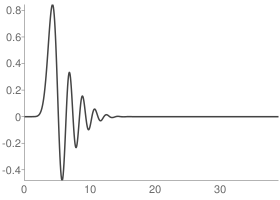
\includegraphics[width=2in]{dbscaling}
    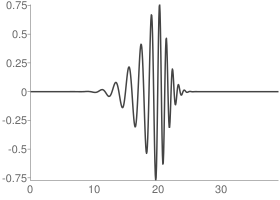
\includegraphics[width=2in]{dbwavelet}  
   \caption{The scaling function $\varphi$ (left) and the wavelet function $\Psi$ (right) }
   \label{fig:wavelet}
\end{figure}

% A pseudo code in python to implement the method:
%\begin{python}
%pip install pywavelet
%\end{python}
%\begin{python}
%import pywt
%import numpy as np
%container = []
%mother_wavelet = 'db20'
%ref_cA, ref_cD = pywt.dwt(ref_sample, mother_wavelet)
%for sample in samples:
%	cA, cD = pywt.dwt(ref_sample, mother_wavelet)
%	cA_dissimilarity = dissimilarity_measure(ref_cA,cA)
%	cD_dissimilarity = dissimilarity_measure(ref_cD,cD)
%	container.append((cA_dissimilarity,cD_dissimilarity))
%\end{python}
\begin{flushleft}
Once we have the two extra features, we compute the dissimilarity between a reference sample and subsequent samples for each feature. 
This process generates a set of points $(x,y)$ that represent the health index of each sample. From Figure \ref{fig:wo} and \ref{fig:wi}, we can observe that bearing number four and bearing number three suffer from ball pass frequency outer race and ball pass frequency inner race defect respectively. We can also observe that a bearing can go through three main stages:
\begin{enumerate}
\item A healthy stage characterised by a low health index
\item A warning stage characterised by an increasing health index
\item An alarm stage characterised by a high health index
\end{enumerate}


\begin{figure}[H] %  figure placement: here, top, bottom, or page
   \centering
   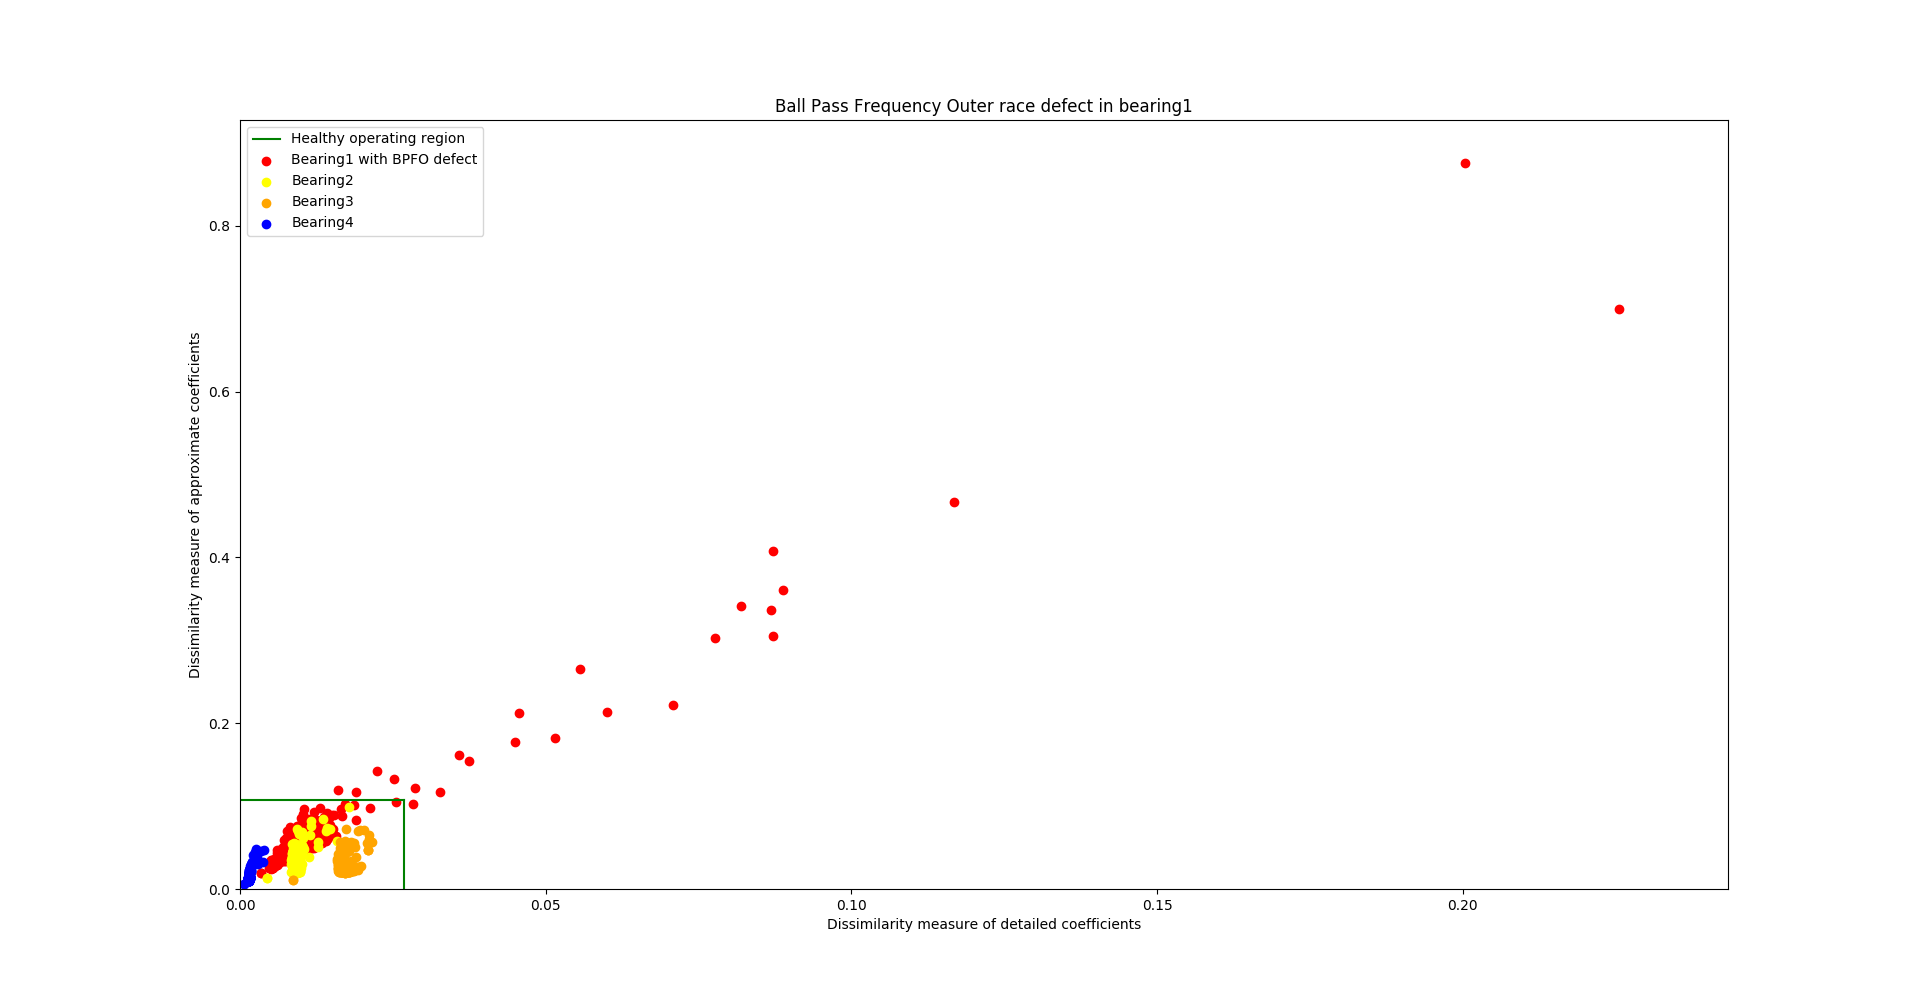
\includegraphics[width=6in]{mixed_method_bpfo.png} 
   \caption{Ball past frequency outer race defect detection from wavelet transform}
   \label{fig:wo}
\end{figure}
\begin{figure}[H] %  figure placement: here, top, bottom, or page
   \centering
   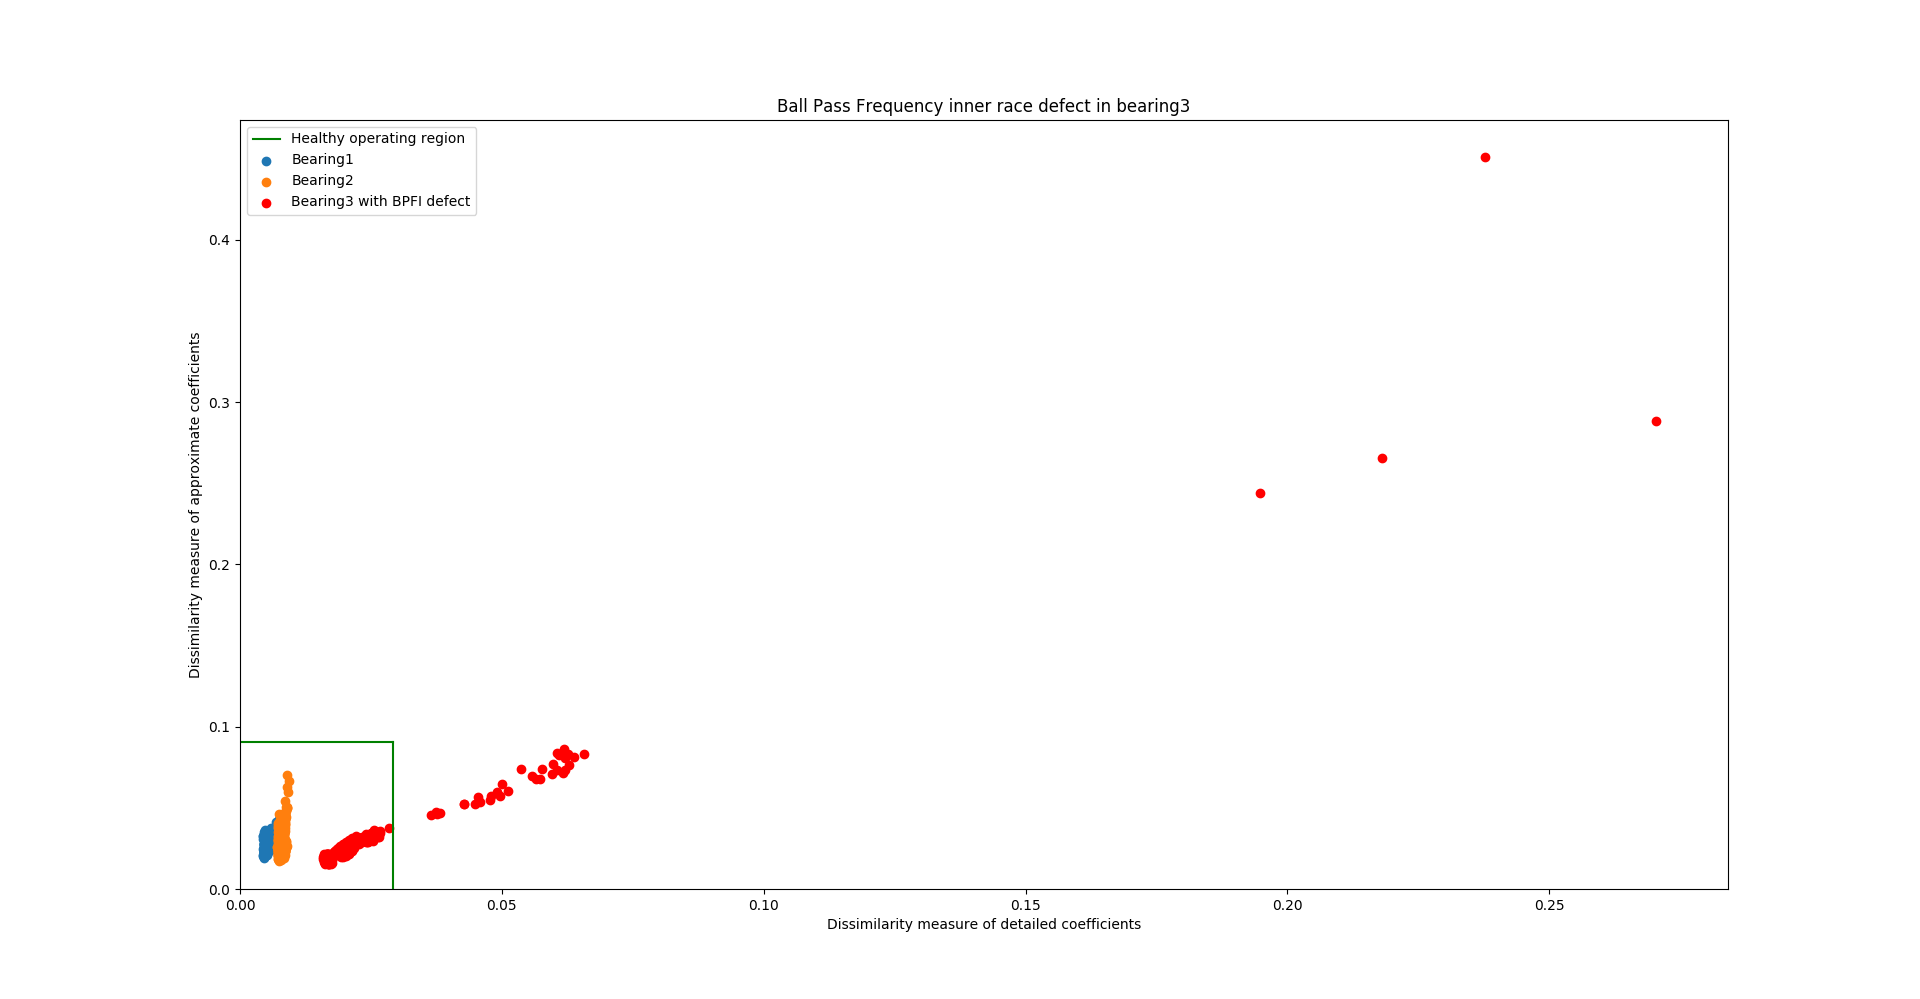
\includegraphics[width=6in]{mixed_method_bpfi.png} 
   \caption{Ball past frequency outer race defect detection from wavelet transform}
   \label{fig:wi}
\end{figure}
In the alarm stage, as the degradation becomes more severe, the distance between the points increases.
\end{flushleft}




%%%%%%%%%%%%%%%%%%%%%%%%%%%%%%%%%%%%%%%%%%%%%%%%%%%%%%%%%%%%%%%%%%%%%%%%%%%%%%%%%%%
%%%%%%%%%%%%%%%%%%%%%%%%%%%%%%%%%%%%%%%%%%%%%%%%%%%%%%%%%%%%%%%%%%%%%%%%%%%%%%%%%%%
\subsection{Hilbert Huang transform}
\subsubsection{Theory}
The Hilbert-Huang transform is a data decomposition methods that consists of decomposing data in an adaptive fashion. Adaptivity means that rather than imposing an a priory basis such as trigonometric functions, a posteriori basis functions are derived from the data itself \cite{norden2008}. In doing so, the method deals better with nonlinearity and non stationarity which are inherently present in real world data.

\begin{flushleft}
This method gives an alternative approach of time-frequency-energy paradigm by using Hilbert spectral analysis and the so call empirical mode decomposition (EMD) to express the nonlinearity and the non stationary in data 
with instantaneous frequency and instantaneous amplitude \cite{norden2008}.
\end{flushleft}
\begin{flushleft}
The empirical mode decomposition (EMD) originated from the quest of functions that can be expressed by a time-frequency-amplitude expression, such that the frequency is physically meaningful.
Consider a time series $x(t)$. Its Hilbert transform H(t) is given by 

\begin{equation}
H(t) = \frac{1}{\pi}P\int_{_\infty}^{\infty}\frac{x(\tau)}{t-\tau}\mathrm{d}\tau,
\end{equation}
where $P$ is the Cauchy principal value. The corresponding time-frequency-amplitude function of $x(t)$ is the analytical function
\begin{equation}
z(t) = x(t) + iy(t) = a(t)e^{i\theta(t)},
\end{equation}
where the instantaneous amplitude $a(t)$ and phase $\theta(t)$ can be computed by 
\begin{equation}\label{eq:amp}
a(t) = \sqrt{x(t)^{2}+ y(t)^{2}}
\end{equation}
\begin{equation}
\theta(t) = \tan^{-1}\left(\frac{y(t)}{x(t)}\right).
\end{equation}
Furthermore, the instantaneous frequency $w(t)$ can be derived from the phase $\theta(t)$ as
\begin{equation}\label{eq:freq}
w(t) = \frac{d\theta}{dt}.
\end{equation}
By setting 
\begin{equation}
f(t) = \frac{y(t)}{x(t)}, \nonumber
\end{equation}
the expression of the instantaneous  amplitude $w(t)$ in (\ref{eq:freq}) can be expanded as
\begin{equation}
w(t) = \frac{f^{\prime}(t)}{1+f(t)^{2}} = \frac{y^{\prime}(t)x(t)-y(t)x^{\prime}(t)}{x(t)(x(t)+y(t)^{2})}.
\end{equation}
The instantaneous frequency $w(t)$ using the Hilbert transform is not always physically meaning. For example for an arbitrarily function, the instantaneous physical frequency values should be positive. However this is not always the case. 

\begin{flushleft} 
For example if 
\begin{equation}
f(x) = \cos(ct) +d 
\end{equation}
where $c$ and $d$ are constants, the instantaneous frequency is given by
\begin{equation}
w(t) = \frac{-c\sin(ct)}{1+(\cos(ct) +d)^{2} }
\end{equation}
\begin{figure}[H] %  figure placement: here, top, bottom, or page
   \centering
   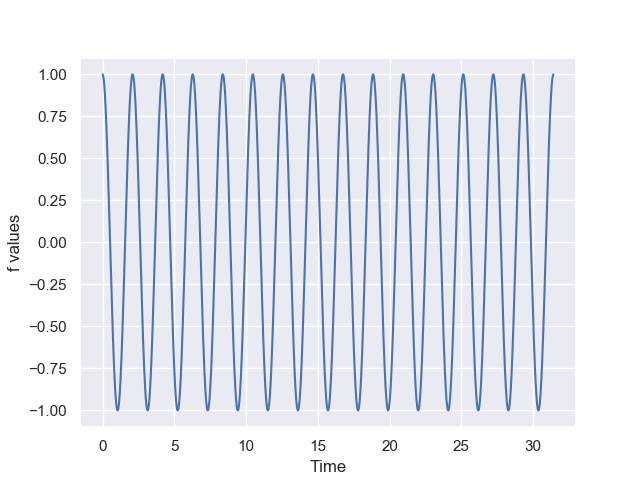
\includegraphics[width=2.5in]{f} 
     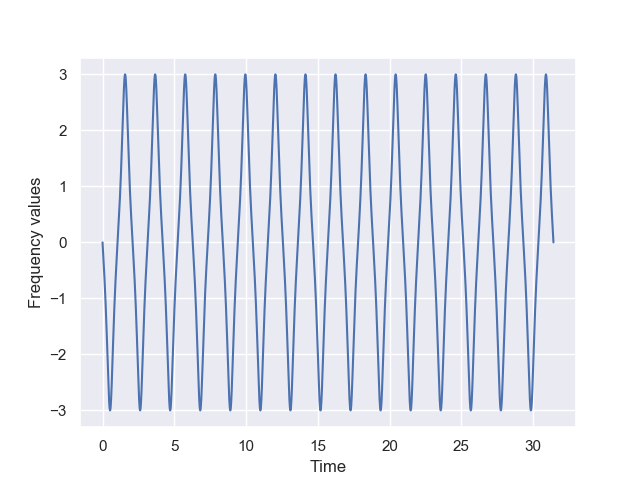
\includegraphics[width=2.5in]{frequency} 
   \caption{function f and its corresponding frequency}
   \label{fig:freq}
\end{figure}
From Figure \ref{fig:freq}, we see that the instantaneous frequency takes negative values, which is not physically meaning full. 
\end{flushleft}

\begin{flushleft}
To circumvent this, the Hilbert-Huang transform offers a methodology to obtain from an arbitrarily function or time series $x(t)$ a set of finite subcomponents whose instantaneous frequency are physically meaningful. This methodology let to the empirical mode decomposition.
\end{flushleft}



%Once the instantaneous frequency and amplitude are defined, we can define the Hilbert-Huang spectrum H(w,t), \cite{hui2007} as 
%\begin{equation}\label{eq:hs}
%H(w,t) = Re\sum_{i=1}^{n}a_{i}(t)\exp\left(\int w_{i}(t)\mathrm{d}t\right),
%\end{equation}
%and compute the marginal spectrum 
%\begin{equation}
%h(w) = \int_{0}^{T}H(w,t)\mathrm{d}t.
%\end{equation}
%While the Hilbert spectrum is the energy contribution of each instantaneous frequency, the marginal spectrum is the total energy contribution of all instantaneous frequency
%\cite{norden2008, hui2007}. 
\end{flushleft}

\begin{flushleft}
 The necessary condition for obtaining a physical frequency is that $x(t)$ satisfies the approximate local envelope symmetry condition \cite{norden1998}. 



This condition 
is expressed in the empirical mode decomposition (EMD) such that an arbitrarily time series $x(t)$ can be decomposed by a sifting process into intrinsic mode function $c_{i}$
\begin{equation}
x(t) = \sum_{i=1}^{n}c_{i} + r_{n}
\end{equation}
where the $c_{i}$ satisfies the approximate local envelope symmetry condition
\begin{equation}
SD_{k} = \frac{\sum_{t=0}^{T}}{\sum_{t=0}^{T}} < \epsilon
\end{equation}
where $\epsilon$ is a small predefined real number.
\end{flushleft}

\subsubsection{Application for bearings fault detection}
we consider a vibration signal with sample frequency of 20000Hz rotating speed of 2000 RPM
\begin{figure}[H] %  figure placement: here, top, bottom, or page
   \centering
   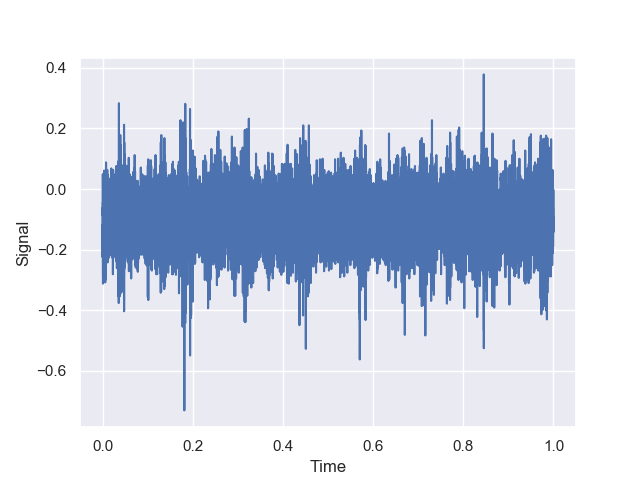
\includegraphics[width=4in]{signal} 
   \caption{Vibration signal of 1 second snapshot}
   \label{fig:signal}
\end{figure}
\begin{flushleft}
After applying the empirical mode decomposition on the vibration data from figure \ref{fig:signal} we get sixteen  intrinsic mode functions
\begin{figure}[H] %  figure placement: here, top, bottom, or page
   \centering
   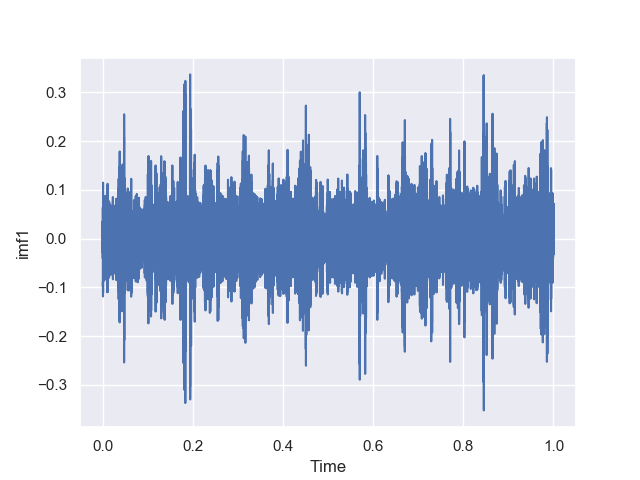
\includegraphics[width=2.5in]{imf/imf1.png} 
     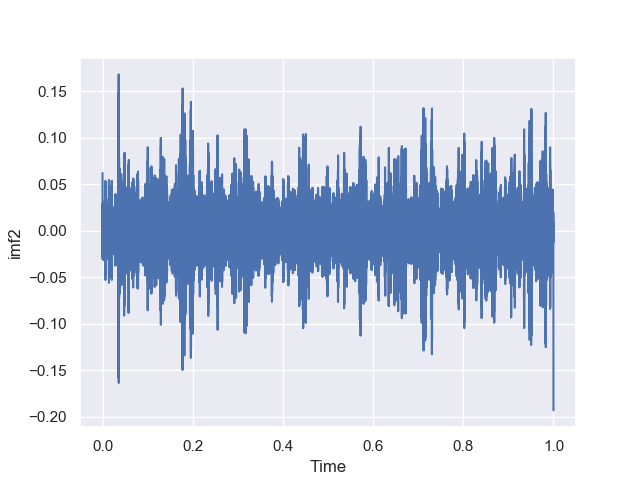
\includegraphics[width=2.5in]{imf/imf2.png} 
   \caption{1th and 2nd intrinsic mode function (imf)}
   \label{fig:imf11}
\end{figure}

\begin{figure}[H] %  figure placement: here, top, bottom, or page
   \centering
   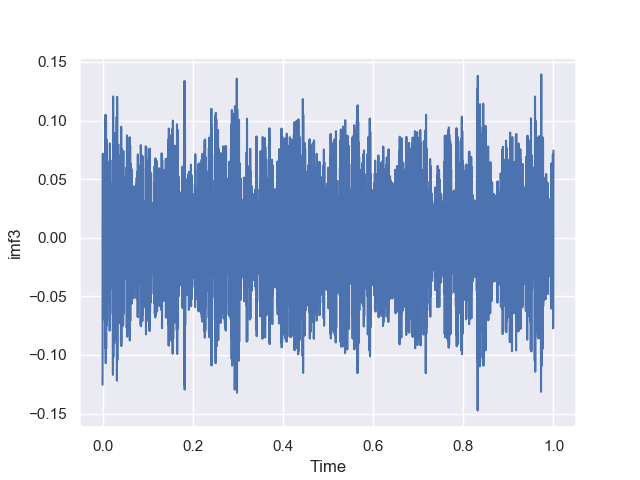
\includegraphics[width=2in]{imf/imf3.png} 
     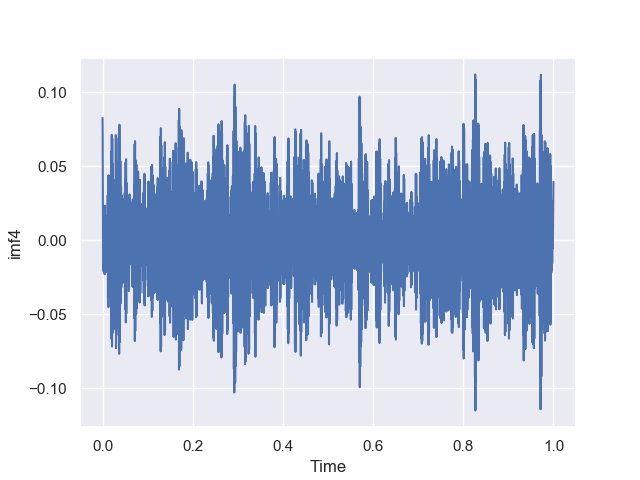
\includegraphics[width=2in]{imf/imf4.png} 
   \caption{3rd and 4th intrinsic mode function (imf)}
   \label{fig:imf34}
\end{figure}

\begin{figure}[H] %  figure placement: here, top, bottom, or page
   \centering
   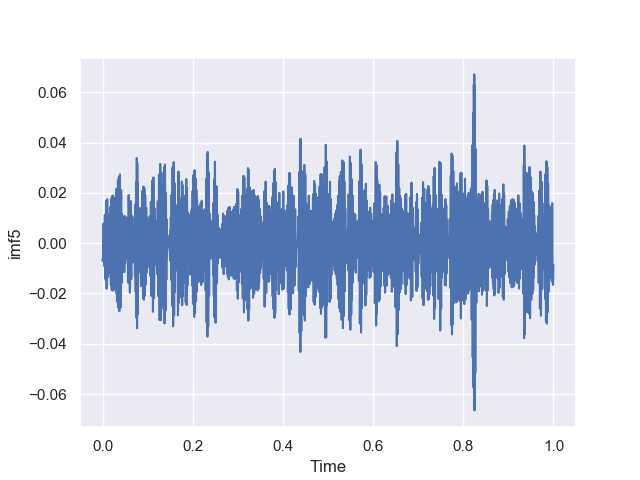
\includegraphics[width=2in]{imf/imf5.png} 
     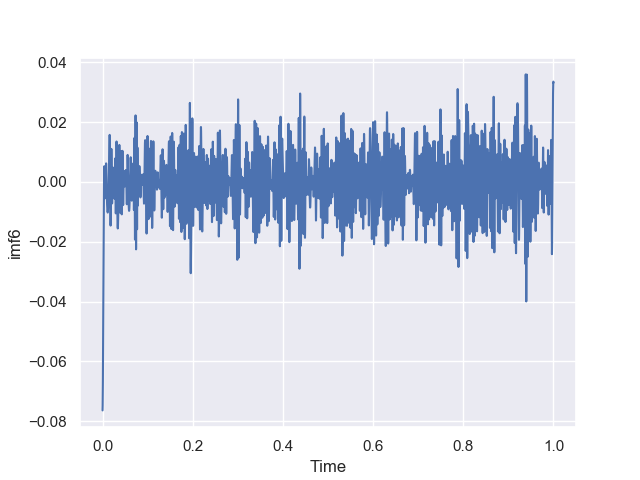
\includegraphics[width=2in]{imf/imf6.png} 
   \caption{5th and 6th intrinsic mode function (imf)}
   \label{fig:imf56}
\end{figure}

\begin{figure}[H] %  figure placement: here, top, bottom, or page
   \centering
   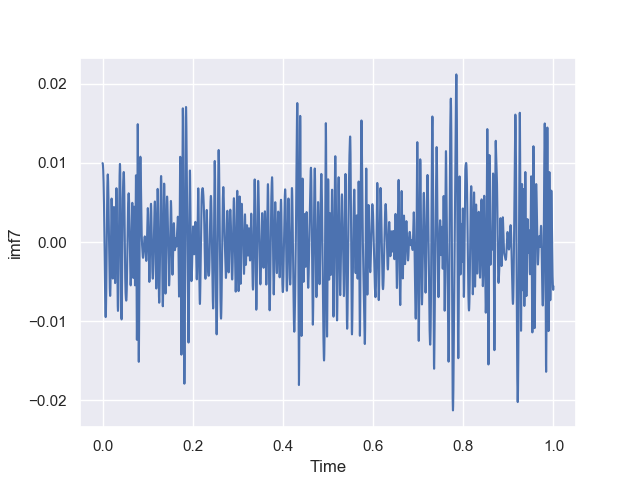
\includegraphics[width=2in]{imf/imf7.png} 
     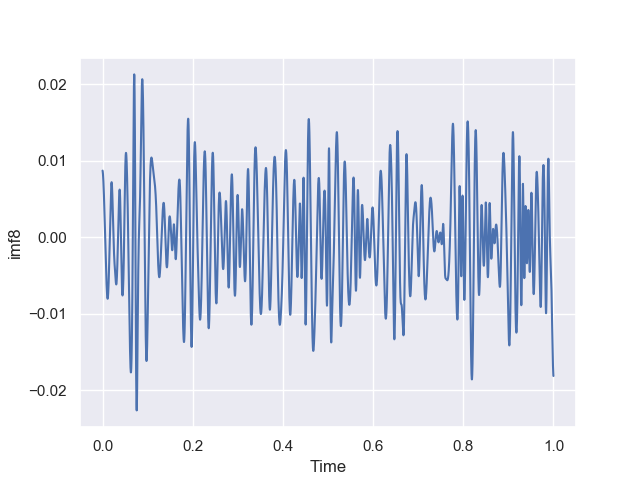
\includegraphics[width=2in]{imf/imf8.png} 
   \caption{7th and 8th intrinsic mode function (imf)}
   \label{fig:imf78}
\end{figure}

\begin{figure}[H] %  figure placement: here, top, bottom, or page
   \centering
   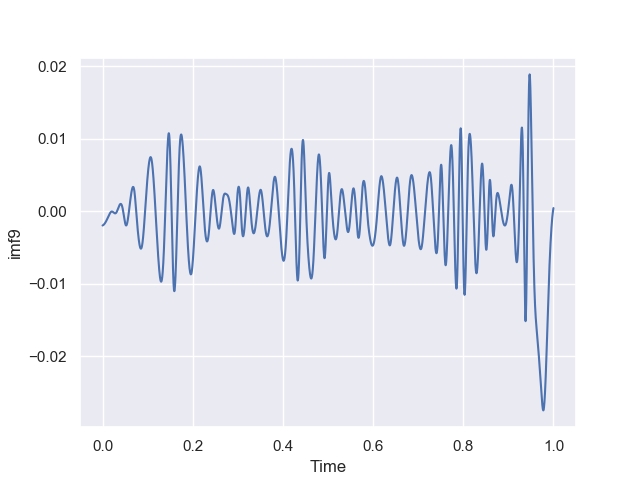
\includegraphics[width=2in]{imf/imf9.png} 
     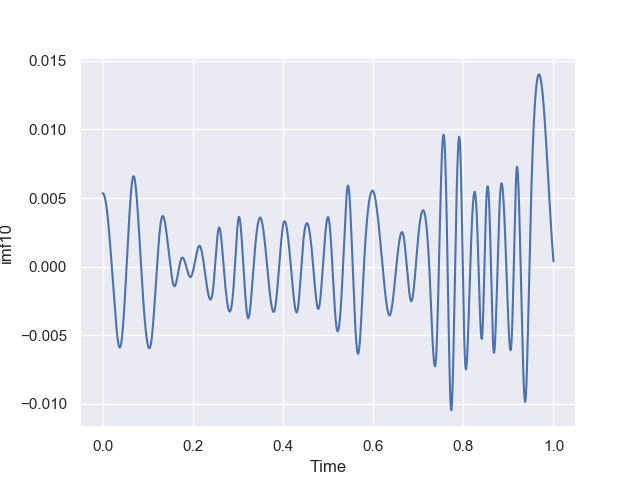
\includegraphics[width=2in]{imf/imf10.png} 
   \caption{9th and 10th intrinsic mode function (imf)}
   \label{fig:imf910}
\end{figure}

\begin{figure}[H] %  figure placement: here, top, bottom, or page
   \centering
   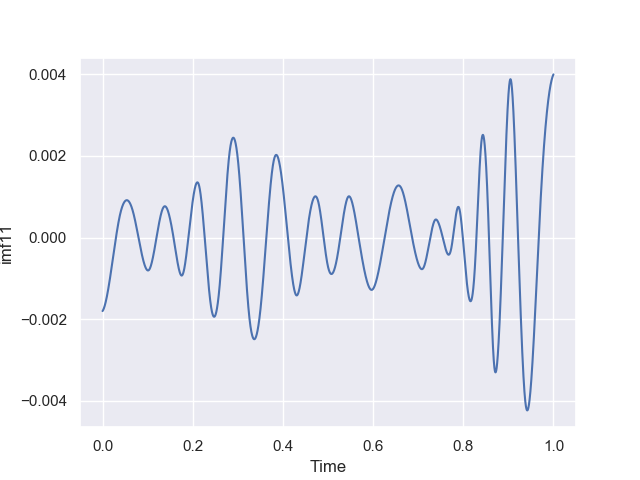
\includegraphics[width=2in]{imf/imf11.png} 
     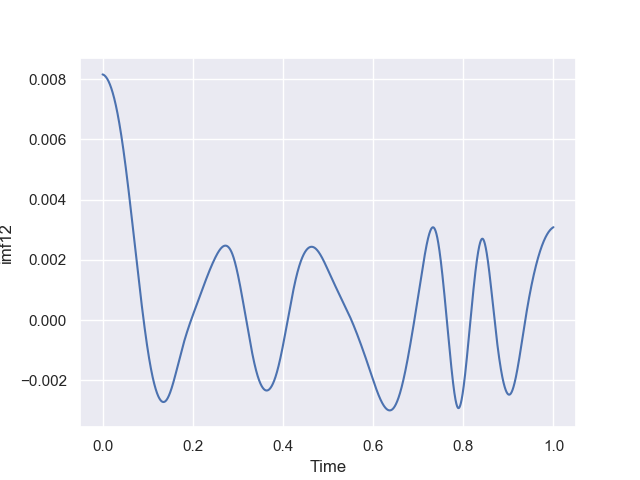
\includegraphics[width=2in]{imf/imf12.png} 
   \caption{11th and 12th intrinsic mode function (imf)}
   \label{fig:imf1112}
\end{figure}

\begin{figure}[H] %  figure placement: here, top, bottom, or page
   \centering
   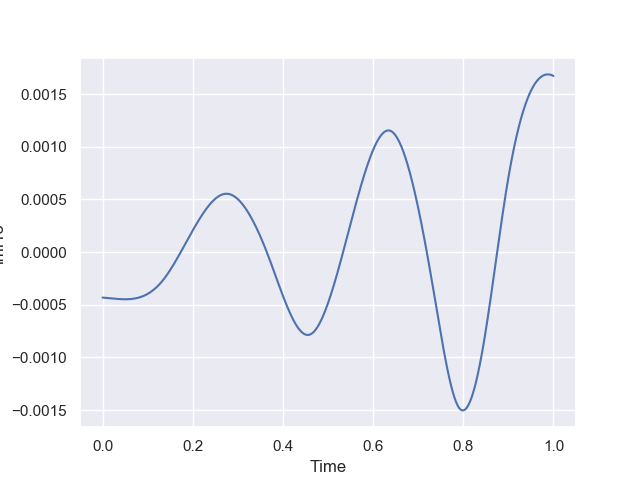
\includegraphics[width=2in]{imf/imf13.png} 
     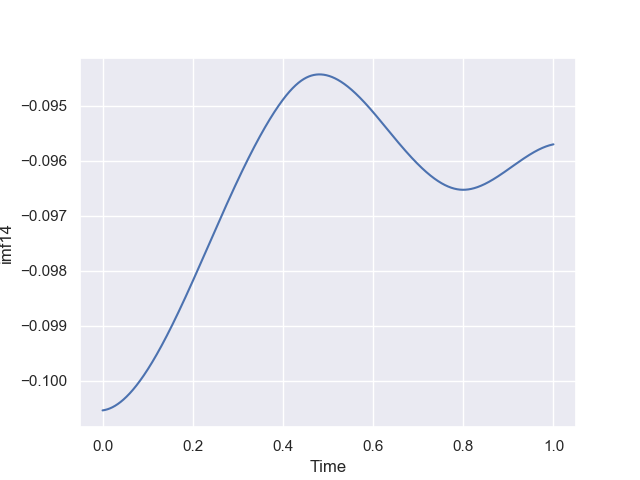
\includegraphics[width=2in]{imf/imf14.png} 
   \caption{13th and 14th intrinsic mode function (imf)}
   \label{fig:imf1314}
\end{figure}

\end{flushleft}


%%%%%%%%%%%%%%%%%%%%%%%%%%%%%%%%%%%%%%%%%%%%%%%%%%%%%%%%%%%%%%%%%%%%%%%%%%%%%%%%%%%%
\section{Machine learning methods   \textcolor{red}{(TO DO!!)}}
\subsection{Overview   \textcolor{red}{(TO DO!!)}}

%%%%%%%%%%%%%%%%%%%%%%%%%%%%%%%%%%%%%%%%%%%%%%%%%%%%%%%%%%%%%%%%%%%%%%%%%%%%%%%%%%%%
%%%%%%%%%%%%%%%%%%%%%%%%%%%%%%%%%%%%%%%%%%%%%%%%%%%%%%%%%%%%%%%%%%%%%%%%%%%%%%%%%%%%



\section{Application of signal processing and machine learning: Case study   \textcolor{red}{(TO DO!!)}}
\subsection{Overview   \textcolor{red}{(TO DO!!)}}
%We apply the methodology described in this work to an application for bearing fault detection.
%\begin{figure}[H] %  figure placement: here, top, bottom, or page
%   \centering
%   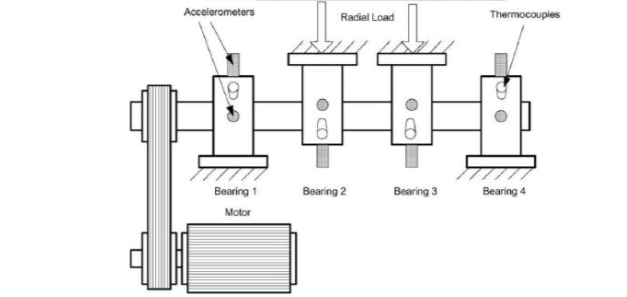
\includegraphics[width=4in]{experiment} 
%   \caption{Experimental set up}
%   \label{fig:exp}
%\end{figure}
%The data used in this use case was generated by the Intelligence Maintenance system (IMS) [link to the IMS].
%Three separate experiments involving four bearings were performed on a motor. In each experiment, a 1-second vibration signal snapshots was recorded every 10 minutes, for a specified time. Each vibrational signal sample consists of 20 480 data points with sampling rate of 20 000 Hz.
%In this post I will be using the first and the second experiment data [available here (give a link to the data)].


\section{Conclusion   \textcolor{red}{(TO DO!!)}}
\begin{thebibliography}{9}
\bibitem{norden2008} 
Norden E. Huang and Zhaohua Wu 
\textit{A review on Hilbert-Huang Transform: Methods and its Application to Geophysical Studies}. 
Review of Geophysics, 2008
 
\bibitem{norden1998} 
Norden E. Huang, Zheng Shen, Steven R. Long, Manlic C. Wu, Hsing H.Shih, Quanan Zheng, Nai-Chyuan Yen, Chi Chao Tung and Henry H. Liu
\textit{The Empirical mode decomposition and the Hilbert Spectrum for nonlinear and non-stationary time series analysis}
Proc. R. Soc. Lond. A (1998) 455, 903:995.

\bibitem{chandola} 
Varun Chandola, Arindam Banerjee, and Vipin Kumar.
\textit{Anomaly detection: A survey}
Proc. R. Soc. Lond. A (1998) 455, 903:995.


 
\bibitem{pwc} 
Michel Mulders and Mark Haarman
\textit{Predictive maintenance 4.0. Predict the unpredictable, June 2017}

 
\bibitem{hui2007} 
Hui Li, Yuping Zhang and Haiqi Zheng
\textit{Hilbert-Huang transform and marginal spectrum for detecting and diagnosis of localized defects in roller bearings}
Journal of Mechanical Technology, 2007
\end{thebibliography}






\end{document}  